\clearpage

\section{Binary To Ascii}

\begin{tcolorbox}	
	\begin{tabular}{p{2.75cm} p{0.2cm} p{10.5cm}} 	
		\textbf{Header File}   &:& binary\_to\_ascii\_*.h \\
		\textbf{Source File}   &:& binary\_to\_ascii\_*.cpp \\
        \textbf{Version}       &:& 20180905 (Andr\'e Mourato)
	\end{tabular}
\end{tcolorbox}

\subsection*{Methods}

BinaryToAscii(vector$\langle$Signal *$\rangle$ \&InputSig, vector$\langle$Signal *$\rangle$ \&OutputSig) :Block(InputSig, OutputSig)\{\};
\bigbreak
void initialize(void);
\bigbreak
bool runBlock(void);
\bigbreak

\subsection*{Functional description}

Figure \ref{BinarySignalImage} shows an example of an input signal that can be passed as argument. This signal contains the binary representation of three characters: a, b and c. Each character can be represented by 8 bits, according to the Ascii Table. This signal contains the following stream of bits: $0110000111000101100011$. There are 24 bits in this stream, therefore we can divide it into three segments of 8 bits each. The resulting segments are: $01100001$, $1100010$ and $1100011$. Each of these segments is the binary code of a character. $01100001$ represents the character $a$, $1100010$ represents the character $b$ and $1100011$ represents the character $c$.
The block BinaryToAscii will convert the binary codes into the respective characters. The resulting output signal will be of type Ascii. The output signal to this example, shown in figure \ref{AsciiSignalImage}, contains the characters that can be represented with the previous binary codes.

\begin{figure}[h]
	\centering
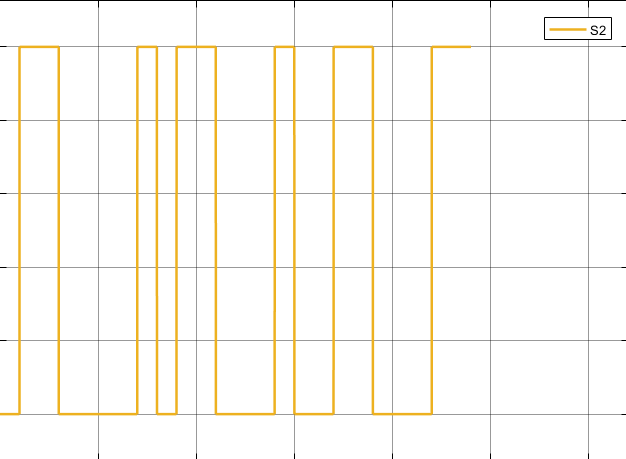
\includegraphics[width=.5\linewidth]{./lib/ascii_to_binary/figures/binary_signal.png}
\caption{Binary signal passed as input to the BinaryToAscii block}\label{BinarySignalImage}
\end{figure}

\begin{figure}[h]
	\centering
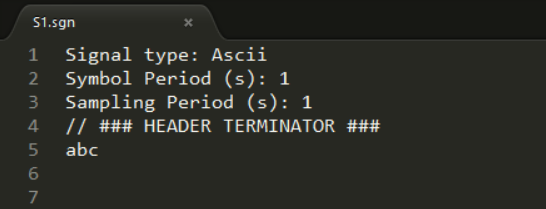
\includegraphics[width=.7\linewidth]{./lib/ascii_to_binary/figures/ascii_signal.png}
\caption{Resulting Ascii signal from the output of the BinaryToAscii block}\label{AsciiSignalImage}
\end{figure}

\pagebreak

\subsection*{Input Signals}

\subparagraph*{Number:} 1

\subparagraph*{Type:} Ascii

\subsection*{Output Signals}

\subparagraph*{Number:} 1

\subparagraph*{Type:} Ascii 